% begin module polar-symmetry
\begin{frame}
\frametitle{Symmetry}
\begin{itemize}
\item<1-| alert@2>  If the polar equation is unchanged when $\theta$ is replaced by $-\theta$, the curve is symmetric about the polar axis.
\item<1-| alert@3>  If the equation is unchanged when $\theta$ is replaced by $\pi + \theta$, the curve is symmetric under rotation about the pole.
\item<1-| alert@4>  If the equation is unchanged when $\theta$ is replaced by $\pi - \theta$, the curve is symmetric about the vertical line $\theta = \frac{\pi}{2}$. 
\end{itemize}
\begin{center}
\ \only<handout:1| -2>{%
\uncover<2>{%
\ 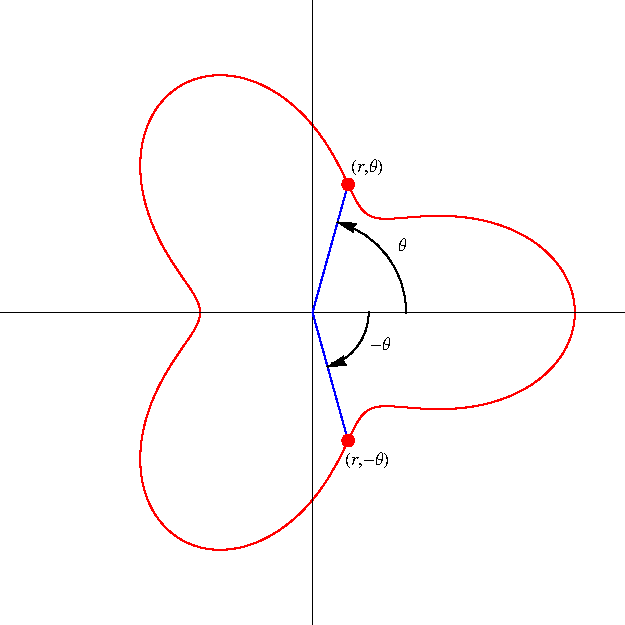
\includegraphics[height=5cm]{polar-curves/pictures/11-03-symmetrya.pdf}%
}}%
\only<handout:2| 3>{%
\ 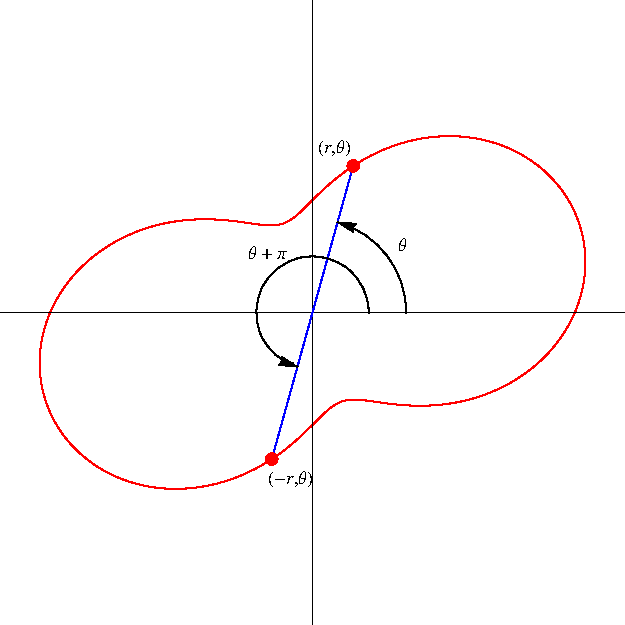
\includegraphics[height=5cm]{polar-curves/pictures/11-03-symmetryb.pdf}%
}%
\only<handout:3| 4->{%
\ 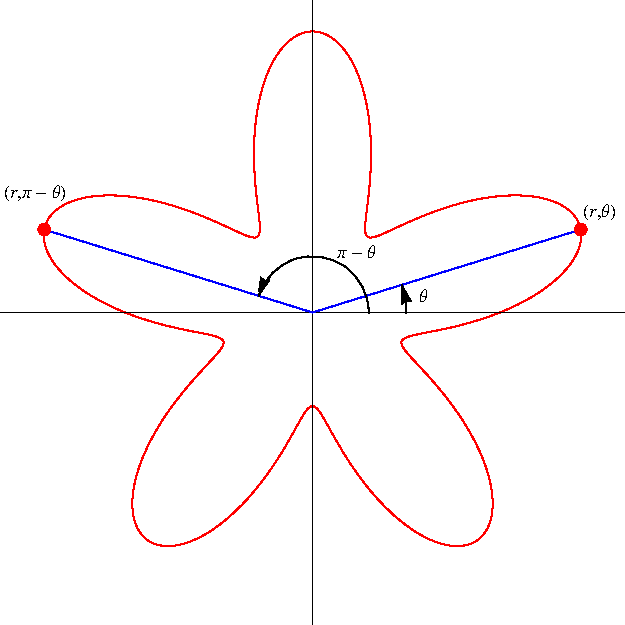
\includegraphics[height=5cm]{polar-curves/pictures/11-03-symmetryc.pdf}%
}
\end{center}
\end{frame}
% end module polar-symmetry
